\documentclass[main.tex]{subfiles}
\begin{document}

\section{Voting}

\subsection{Voting Process and States}

As shown in figure \ref{fig:FSM}, you can consider each DARC protocol as a finite-state machine (FSM) with three states:

1. Idle state: In this state, the DARC protocol can accept any program. When a program is accepted and executed, the DARC protocol transitions back to the idle state. Similarly, if a program is rejected, the DARC protocol returns to the idle state. When a program contains an operation that requires voting, the DARC protocol transitions to the voting state.

2. Voting state: During the voting state of the DARC Protocol, all users are allowed and exclusively permitted to execute programs containing a single vote operation. If a program contains multiple operations, the program will be rejected. Similarly, if a program contains a single operation that is not a vote, the program will also be rejected. If the current vote is approved, the system will automatically transition to the execution pending state. Additionally, the voting state has a minimum time limit. If, within this time limit, the supporting votes for each voting item do not collectively exceed the defined threshold, the current voting round is considered unsuccessful, and the system will automatically return to the idle state. Only when all voting items receive approval within the specified time limit will the program be approved by the DARC protocol.

3. Execution pending state: When a program is voted upon and approved by the DARC protocol, it can be executed in the execution pending state. The execution pending state also has a minimum time limit. If the program is executed within this limit, it will be successfully executed, and the system will automatically revert to the idle state. If execution does not occur within this limit, the program will fail to execute, and the DARC protocol will discard the program, automatically returning to the idle state.

\begin{figure}
\centering
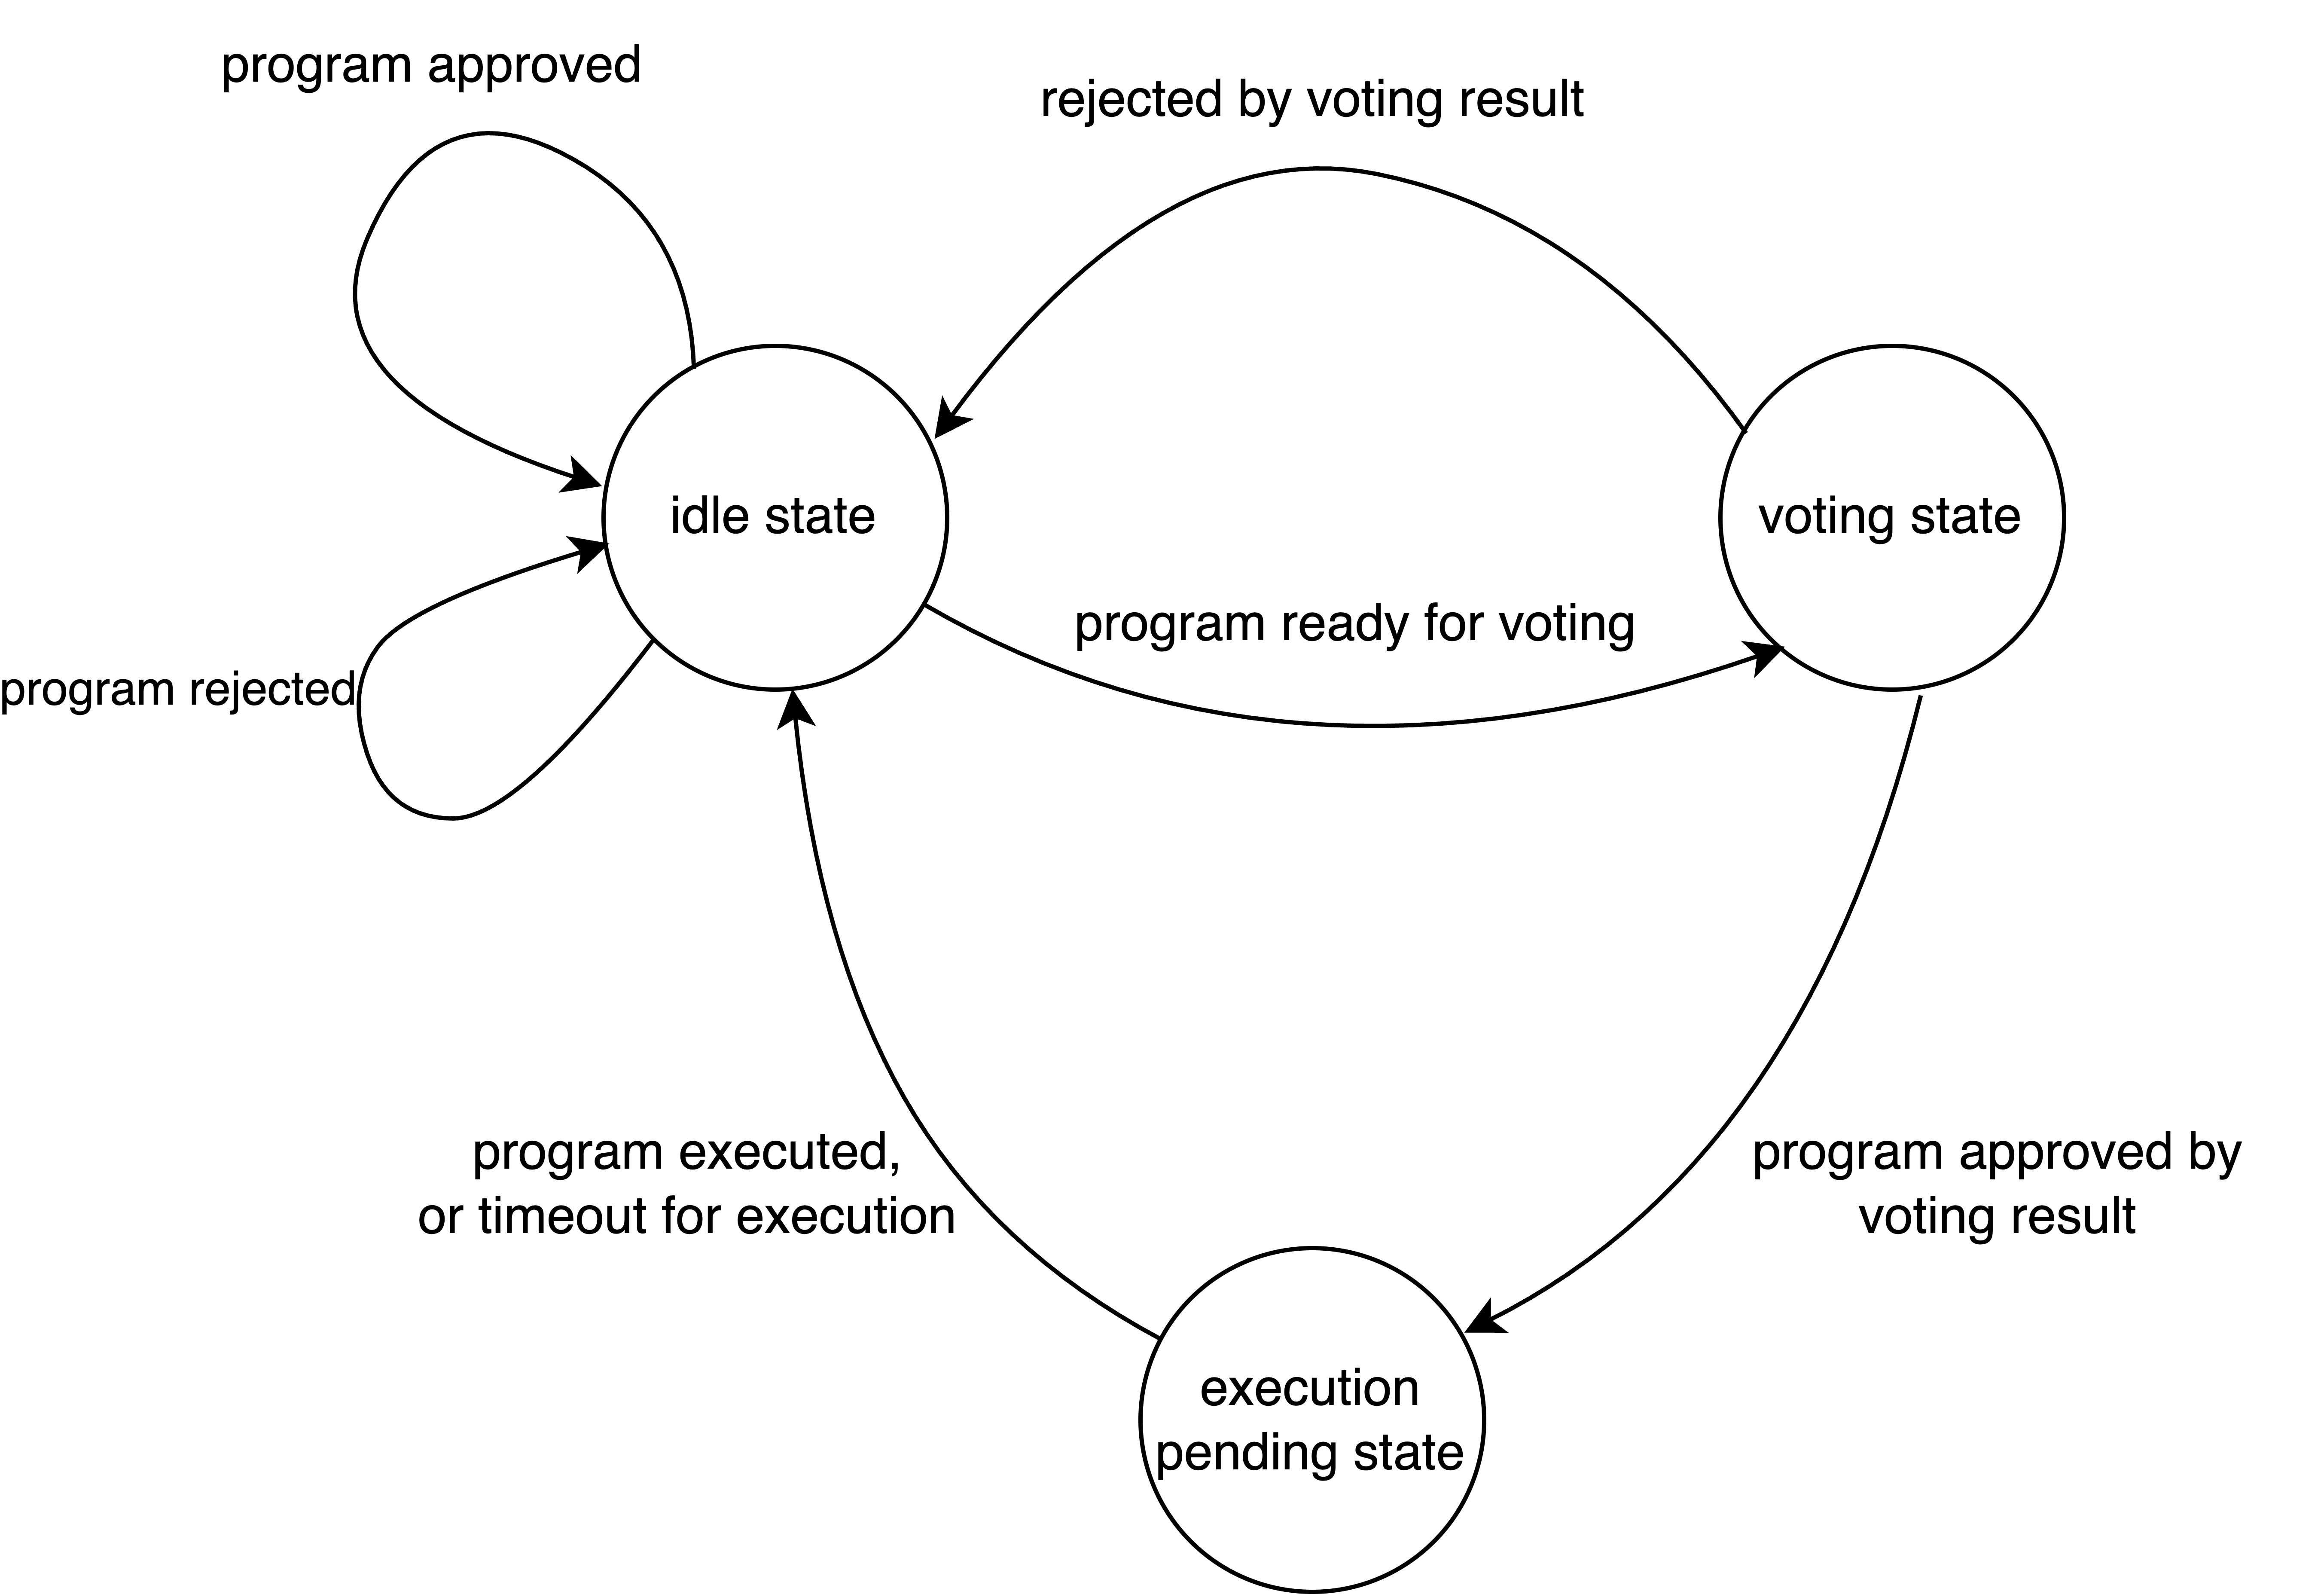
\includegraphics[width=1\linewidth]{finite_state_machine.drawio.large.png}
\caption{\label{fig:FSM}The finite-state machine of DARC}
\end{figure}

\subsection{Voting Rules}

Each voting rule is composed with following items:
\begin{itemize}
    \item Voting token class list: a list of token class indices that are allowed to vote for this voting item. It contains at least one valid token class index number. All tokens with indices listed in this array are considered as valid voting tokens. All token holders that holds any tokens that are included in this array are allowed to vote for this item.
    \item Approval threshold percentage: the approval threshold in percentage. 
    \item Boolean flag \texttt{bIsAbsoluteMajority}: a boolean flag that indicates if the voting mode is by absolute majority or relative majority.
    \item Voting duration(in seconds): the maximum duration for this voting process in seconds. If the voting process takes more time than this parameter, the voting process will be terminated and the vote result will be set as failure.
    \item Executing pending duration(in seconds): the maximum duration for the operator to execute an approved program after a voting process finishes. If the program is approved, the operator must execute this program in a certain period of time, otherwise the program will be aborted and the DARC will be reset to idle state.
    \item Boolean flag \texttt{isForceStopAllowed}: If this flag is set as \texttt{True}, some operators can stop this voting process manually.
    \item Boolean flag \texttt{isEnabled}: a boolean flag that must be set as \texttt{True} if the voting rule is initialized and enabled successfully.
    \item Note: a string stored in the voting rule with extra information, comments or external URLs about this voting rule.
\end{itemize}

\begin{verbatim}
struct VotingRule {

  /**
   * the voting token class index list
   */
  uint256[] votingTokenClassList;

  /**
   * the approval threshold percentage of the voting policy
   */
  uint256 approvalThresholdPercentage;

  /**
   * the voting duration of the voting policy in seconds
   */
  uint256 votingDurationInSeconds;

  /**
   * the execution pending duration of the voting policy in seconds
   */
  uint256 executionPendingDurationInSeconds;

  /**
   *  the forced stop during the voting duration is allowed or not
   */
  bool isForcedStopAllowed;

  /**
   * the voting policy is enabled or not
   */
  bool isEnabled;

  /**
   * the note of the voting policy
   */
  string note;

  /**
   * the voting policy is absolute majority or relative majority.
   */
  bool bIsAbsoluteMajority;
}
\end{verbatim}


\subsection{Voting Types}

Typically, in the voting system of DARC protocol, there are two types of voting methods:

\begin{itemize}
    \item Absolute Majority: In absolute majority, the approval of a vote requires reaching a fixed threshold. Expressed as a percentage of the total voting weight, if the total weight of approval votes exceeds a predetermined threshold, the vote is considered passed. For example, with a total weight of 1000 and a threshold set at 70\%, the vote is deemed successful only if the total weight of approval votes exceeds 700.

    \item Relative Majority: In relative majority, the approval of a vote is relative to the percentage of the total voting weight. In this case, the total voting weight can be a percentage of the actual cast votes, rather than a predefined absolute value. For instance, if the total weight is 1000 but only 300 weight is cast in the vote, relative majority requires that the approved vote weight exceeds 70\% of the cast votes (0.7 * 300 = 210) for the vote to be considered successful.
\end{itemize}


We present the options of ``absolute majority'' and ``relative majority'' in voting due to the distinct emphases these two modes offer when balancing the outcomes of the vote.

With regards to the Absolute Majority, its advantage is that the approved voting weight only needs to constitute a proportion of the total possible vote, offering more flexibility. It is applicable in situations where a significant majority is sufficient to determine the outcome in order to promote broader consensus. Its application scenario is suitable for important decisions where it is crucial to secure support from a substantial majority. Using an absolute majority as the criterion serves to promote broader consensus.

As for the Relative Majority, its advantage is that the approved voting weight simply needs to constitute the largest share of the current vote, providing greater expediency and flexibility. It is thus applicable in situations where a relative majority is sufficient to determine the outcome. Its application scenario is suited for scenarios where a more flexible and expedited decision-making process is required. A relative majority can achieve consensus more quickly without needing to secure a fixed percentage of the total possible voting weight.

By providing both absolute and relative majority options, we enhance the adaptability of voting rules to serve the diverse governance needs of various protocols and organizations. Opting for the appropriate voting mode facilitates better fulfilling the consensus and efficiency requirements of particular decision scenarios.

\subsection{Voting Mechanism}

For each program, after receiving approval from the before-operation plugin and completing its full execution within the sandbox, the judgment system, guided by all after-operation plugins, evaluates each operation. If the judgments from all plugins at the highest level for a particular operation are marked as ``VOTING\_NEEDED'', all the voting rules associated with that plugin are collected. Once the judgment system has compiled all the voting rules corresponding to each operation within the program, it generates a voting item array, assigning each rule to its respective entry.


For each operation, there may be one or more distinct plugins simultaneously triggered, all having a return type of ``VOTING\_NEEDED''. In such cases, the voting rules associated with each plugin pointing to that operation will be gathered in order. On the other hand, for each program, different operations may be successively triggered by the same plugins. In the voting item array, a new voting item will be generated for each operation, pointing to the respective voting rule.

Figure \ref{fig:voting_item} is an example illustrating how the DARC protocol initializes a voting item array based on judgment results.

\begin{figure}
\centering
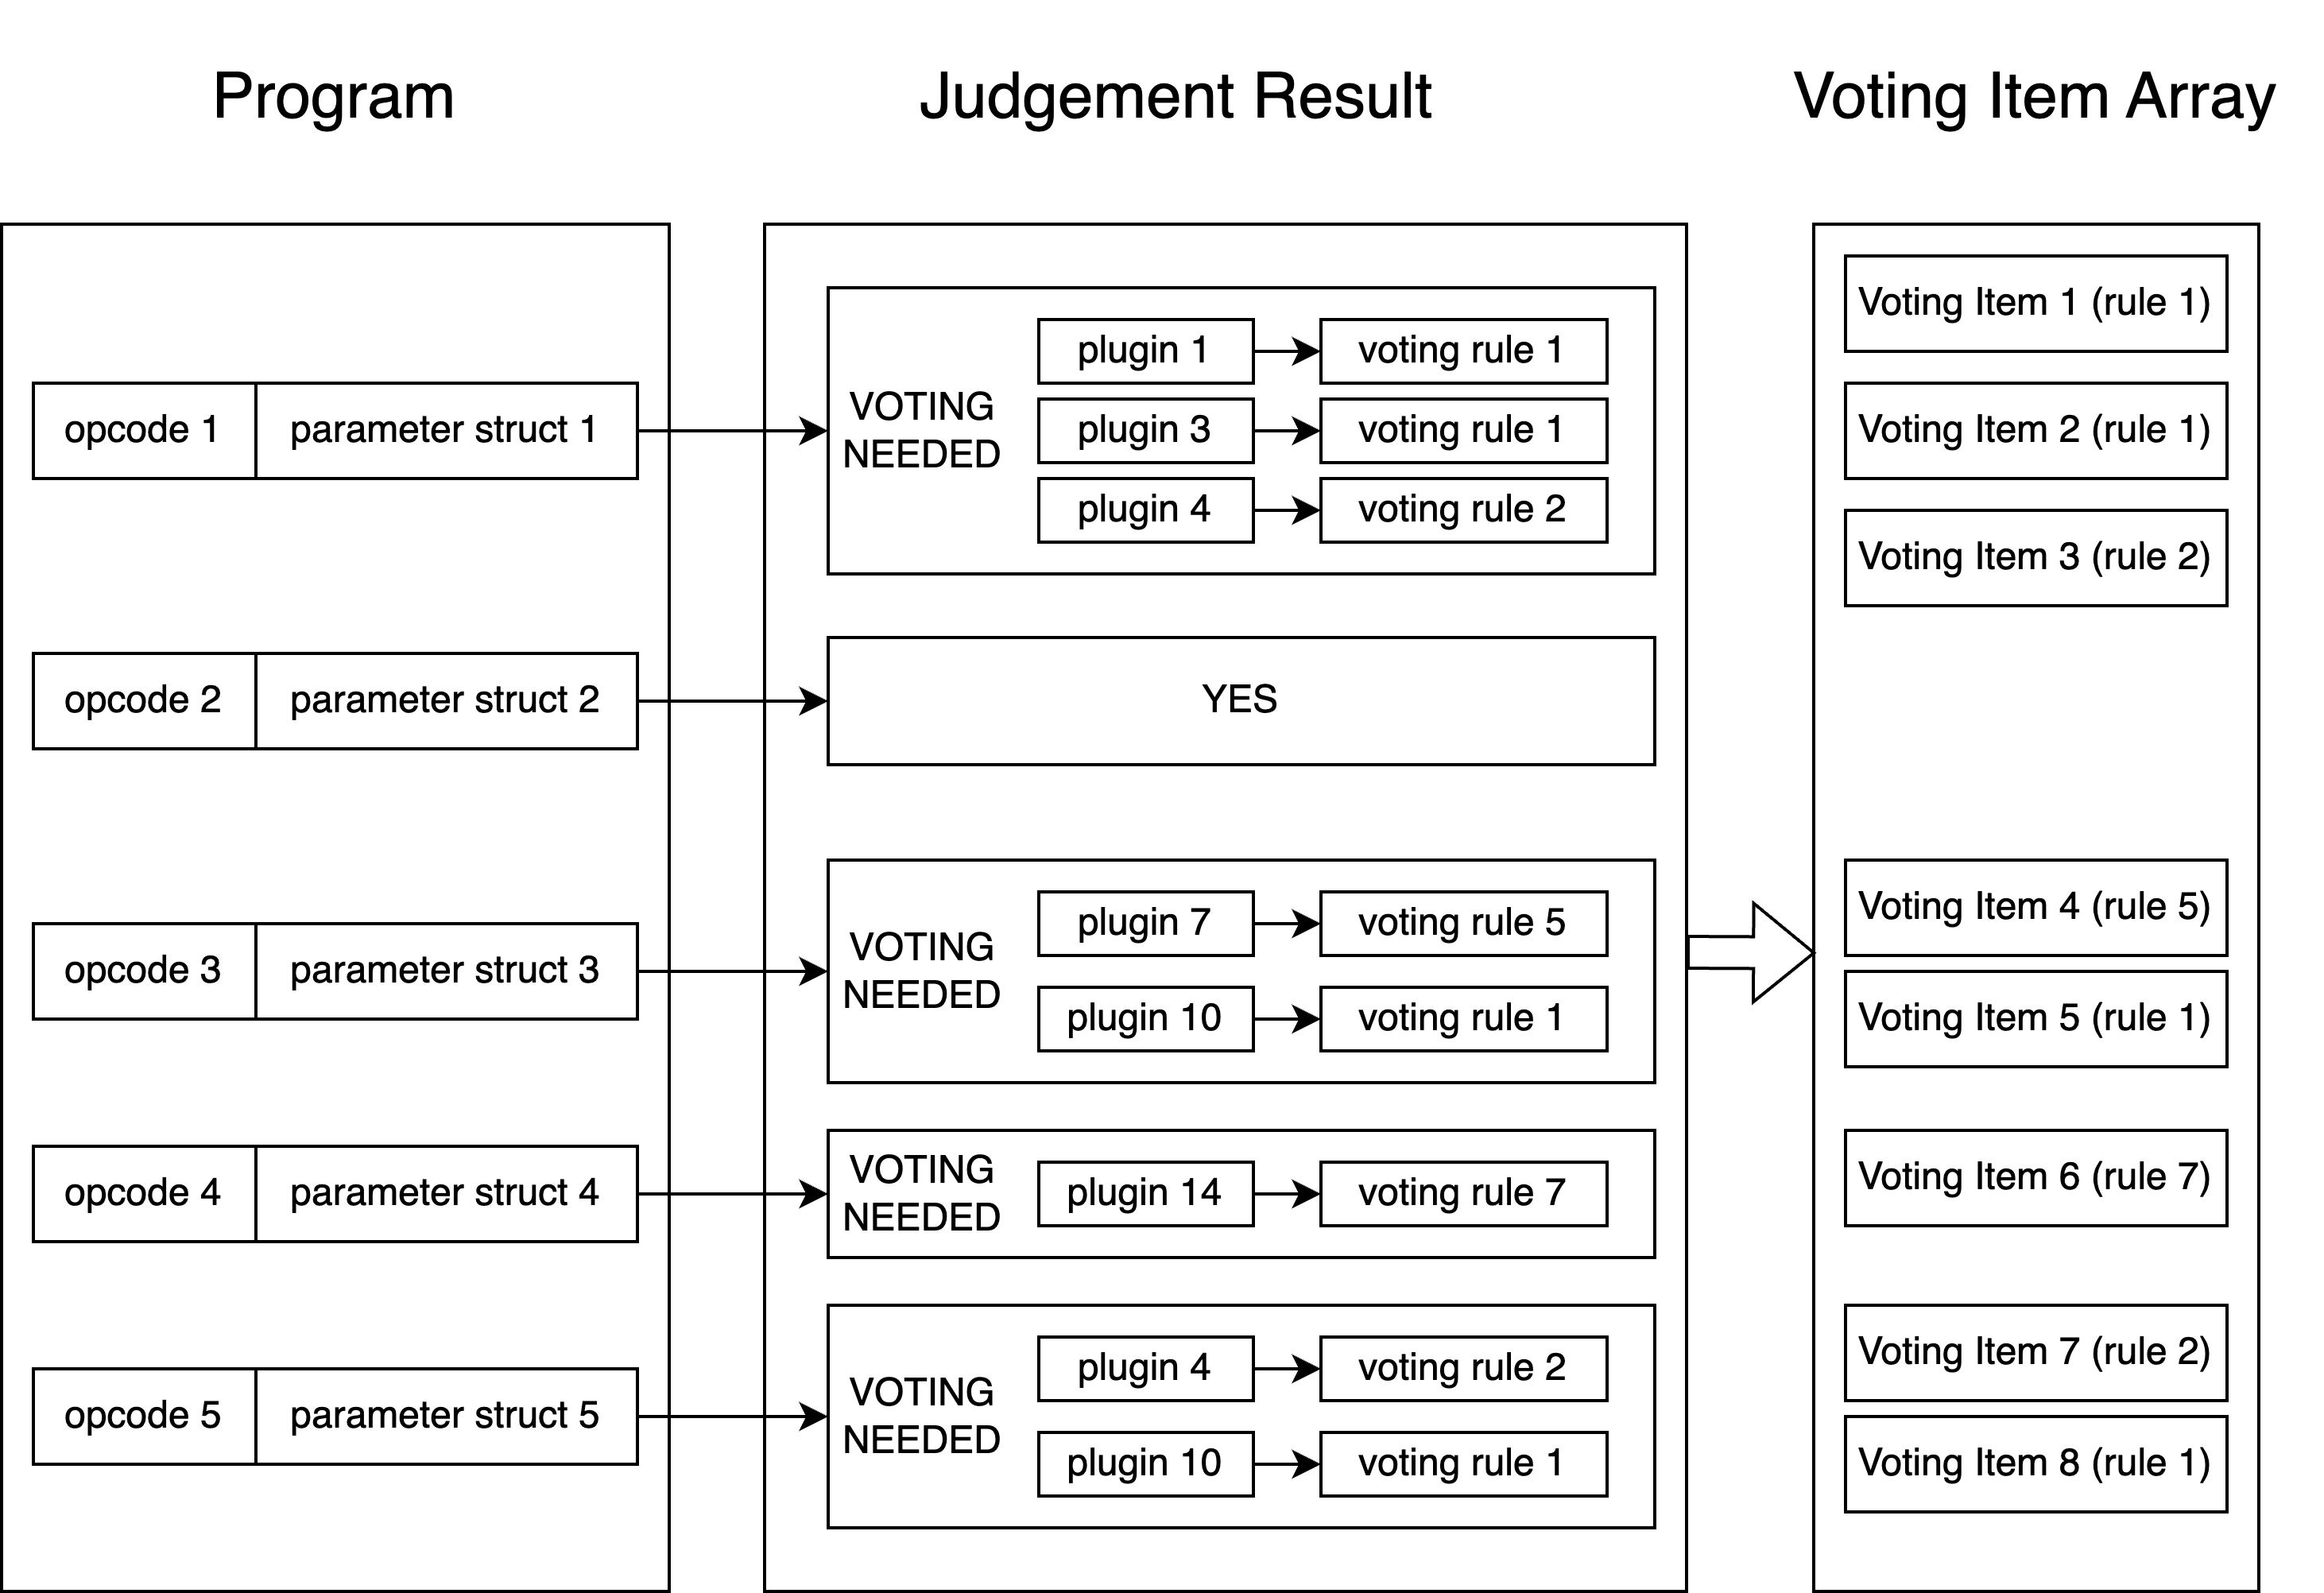
\includegraphics[width=1\linewidth]{voting_item.drawio.png}
\caption{\label{fig:voting_item}Voting Rules and Items}
\end{figure}


Once a voting item array is initialized, as a finite state machine, the DARC protocol transitions into the voting state. Assuming there are N voting items in the voting item array, all operators will be allowed to cast their votes, submitting a boolean array of length N. Each boolean value represents the operator's support or opposition to the corresponding voting item. For each operator, in every voting state, they can and must vote only once, ensuring that the parameter in the vote operation is a boolean array of length N. If an operator attempts to execute a vote operation more than once or provides a boolean array of a length other than N, the voting program will be automatically rejected.

In the DARC protocol, each voting item has two counters: one for ``YES'' votes and another for ``NO'' votes. Whenever an operator performs a valid voting operation, each voting item calculates the total voting weight of that operator in the corresponding voting rule. In a given voting item, each voting rule defines a set of allowed token levels \(C = [c_1, c_2, ..., c_n]\), where \(n\) is the number of token levels. Each token level \(c_i\) has a corresponding voting weight denoted as \(v_i\). Suppose during the voting process, an operator chooses to vote on this voting item, the operator's voting weight \(W\) is calculated by the following formula:

\[
W = \sum_{i=1}^{n} w_i v_i
\]

In this formula, \(W\) represents the total voting weight of the operator for this voting item, and the summation goes through all token levels \(c_i\) allowed for voting. For each level \(i\), \(v_i\) is the quantity of tokens at that level, and \(w_i\) is the corresponding voting weight for level \(i\).

After each operator submits a valid vote operation, each voting item will increment the corresponding voting weight into the YES or NO counters. If the operator holds zero tokens in the votable token set for a particular voting item, neither the YES nor NO counters will be affected. Upon the completion of the voting process, the DARC protocol will determine whether the voting has concluded based on the following criteria:

\begin{enumerate}

    \item When there is at least one voting item among all voting items operating in absolute majority mode, and this voting item has received a sufficient number of NO votes, the entire voting process will terminate prematurely, resulting in a voting failure. Subsequently, the DARC protocol transitions into the idle state. For instance, if a voting item has an approval threshold of 66\%, operates in absolute majority mode, and has collected over 34\% of NO votes before the deadline, the entire voting process will immediately conclude, resulting in a voting failure and transitioning into the idle state.

    \item When all voting items exclusively operate in absolute majority mode, and each voting item has garnered YES votes surpassing the approval threshold, the entire voting process concludes prematurely, indicating a successful vote. Subsequently, the DARC protocol transitions into the execution pending state.
    
    \item When the voting state does not meet criteria 1 and 2, the DARC protocol will wait until the deadline expires for assessment. If, post-deadline, each voting item in absolute majority mode has received equal to or more than the total voting weight multiplied by the threshold in YES votes, and for each voting item in relative majority mode, the item has garnered equal to or more than the submitted voting weight multiplied by the threshold in YES votes, the vote is approved, and the DARC protocol transitions to the execution pending state. If any voting item fails to meet this criterion, the vote is deemed unsuccessful, and the DARC protocol reverts to the idle state.
\end{enumerate}

After entering the execution pending state, the program stored in the current voting state has been approved and is ready for execution. The program must be completed before the new execution pending deadline. Upon successful execution, the DARC protocol transitions to the idle state. However, if an error or exception occurs during execution or if no one executes the program before the deadline, the DARC protocol also reverts to the idle state, and the program becomes unable to proceed with execution.


\end{document}